\documentclass{article}

\usepackage[a4paper]{geometry}

\usepackage[brazil]{babel}
\usepackage[T1]{fontenc}

\usepackage{amsmath}
\usepackage{amssymb}

\usepackage{graphicx}

\usepackage{multicol}

\usepackage{ifthen}

\newcommand{\R}{\mathbb{R}}

\DeclareMathOperator*{\cond}{cond}

% noindent EVERYWHERE
\setlength{\parindent}{0pt}

\newenvironment{question}
    {\medskip\bfseries\large}
    {\medskip}

\newcounter{exe-list}
\newenvironment{exe-list}
    {\begin{list}{(\alph{exe-list})}{\usecounter{exe-list}}}
    {\end{list}}

\newenvironment{exe}[2][Sala]
    {\bigskip\noindent\par\ifthenelse{\equal{#1}{}}%
        {\textbf{\LARGE #2}}%
        {\textbf{\LARGE #1~#2}}%
    \medskip\noindent\par}
    {\bigskip}

\newcommand{\todo}[1]{\textbf{TODO:} {\itshape #1}}
\newcommand{\note}[1]{(\textbf{Nota:} {\itshape #1})}

\newcommand{\hashi}{Daniel Kiyoshi Hashimoto Vouzella de Andrade}
\newcommand{\dre}{119025937}

\title{Lista de Revisão}
\author{\hashi{} -- \dre{}}
\date{Álgebra Linear Aplicada - 2023.1}

\begin{document}
\maketitle

\begin{exe}{1}
    \begin{question}
        Calcule:
        \[
            \min_x \left\|
                a - x \; b
            \right\|^2
        \]
        onde:
        \[
            a = \begin{bmatrix}
                a_0 \\ a_1 \\ a_2
            \end{bmatrix}
            \qquad\text{,}\qquad
            b = \begin{bmatrix}
                1 \\ 1 \\ 1
            \end{bmatrix}
            \qquad\text{e}\qquad
            a_0, a_1, a_2, x \in \R
        \]
    \end{question}

    Da questão \(2\), foi calculado o mínimo
    para \(a\) e \(b\) arbitrários:
    \[
        a^T a - \frac{(b^T a)^2}{b^T b}
    \]

    Substituindo os valores:
    \begin{align*}
        &\begin{bmatrix}
                a_0 \\ a_1 \\ a_2
            \end{bmatrix}^T \begin{bmatrix}
                a_0 \\ a_1 \\ a_2
            \end{bmatrix}
            - \frac{
                \left(\begin{bmatrix}
                    1 \\ 1 \\ 1
                \end{bmatrix}^T \begin{bmatrix}
                    a_0 \\ a_1 \\ a_2
                \end{bmatrix} \right)^2
            }{
                \begin{bmatrix}
                    1 \\ 1 \\ 1
                \end{bmatrix}^T \begin{bmatrix}
                    1 \\ 1 \\ 1
                \end{bmatrix}
            } \\
        &\begin{bmatrix}
                a_0 & a_1 & a_2
            \end{bmatrix} \cdot \begin{bmatrix}
                a_0 \\ a_1 \\ a_2
            \end{bmatrix}
            - \frac{
                \left(\begin{bmatrix}
                    1 & 1 & 1
                \end{bmatrix} \cdot \begin{bmatrix}
                    a_0 \\ a_1 \\ a_2
                \end{bmatrix} \right)^2
            }{
                \begin{bmatrix}
                    1 & 1 & 1
                \end{bmatrix} \cdot \begin{bmatrix}
                    1 \\ 1 \\ 1
                \end{bmatrix}
            } \\
        & a_0^2 + a_1^2 + a_2^2
            - \frac{(a_0 + a_1 + a_2)^2}{3} \\
        & \frac{3 \; a_0^2 + 3 \; a_1^2 + 3 \; a_2^2
            - (a_0^2 + a_1^2 + a_2^2
                + 2 \; a_0 \; a_1
                + 2 \; a_0 \; a_2
                + 2 \; a_1 \; a_2)
            }{3} \\
        & \frac{2 \; a_0^2 + 2 \; a_1^2 + 2 \; a_2^2
            - 2 \; a_0 \; a_1
            - 2 \; a_0 \; a_2
            - 2 \; a_1 \; a_2
            }{3}
    \end{align*}
\end{exe}

\begin{exe}{2}
    \begin{question}
        Calcule:
        \[
            \min_x \left\|
                a - x \; b
            \right\|^2
        \]
        onde:
        \[
            a, b \in \R^n
            \qquad\text{e}\qquad
            x \in \R
        \]
    \end{question}

    \begin{align*}
        &\min_x \left\| a - x \; b \right\|^2 \\
        &\min_x (a - x \; b)^T (a - x \; b) \\
        &\min_x a^T a - x \; b^T a - x \; a^T b + x^2 \; b^T b \\
        &\min_x a^T a - x \; b^T a - x \; b^T a + x^2 \; b^T b \\
        &\min_x a^T a - 2 \; x \; b^T a + x^2 \; b^T b
    \end{align*}

    Derivando expressão interna de \(\min\) em relação à \(x\)
    e igualando a \(0\) (para achar pontos críticos):
    \begin{align*}
        &- 2 \; b^T a + 2 \; x \; b^T b = 0 \\
        &2 \; x \; b^T b = 2 \; b^T a \\
        &x \; b^T b = b^T a \\
        &x = \frac{b^T a}{b^T b}
    \end{align*}

    Dessa forma o mínimo é:
    \begin{align*}
        &a^T a - 2 \; x \; b^T a + x^2 \; b^T b \\
        &a^T a - 2 \; \frac{b^T a}{b^T b} \; b^T a
            + \left(\frac{b^T a}{b^T b}\right)^2 \; b^T b \\
        &a^T a - 2 \; \frac{(b^T a)^2}{b^T b}
            + \frac{(b^T a)^2}{b^T b} \\
        &a^T a - \frac{(b^T a)^2}{b^T b}
    \end{align*}
\end{exe}

\begin{exe}{3}
    \begin{question}
        (Regressão Rigde) Calcule:
        \[
            \min_x \left\|
                A \; x - b
            \right\|^2
            + \lambda \; \|x\|^2
        \]
        onde:
        \[
            A \in \R^{m \times n}
            \qquad\text{,}\qquad
            b \in \R^m
            \qquad\text{,}\qquad
            x \in \R^n
            \qquad\text{e}\qquad
            \lambda \in \R
        \]
    \end{question}

    \begin{align*}
        &\min_x \left\| A \; x - b \right\|^2 + \lambda \; \|x\|^2 \\
        &\min_x (A \; x - b)^T (A \; x - b) + \lambda \; x^T x \\
        &\min_x x^T A^T A \; x - b^T A \; x
            - x^T A^T b + b^T b + \lambda \; x^T x \\
        &\min_x x^T A^T A \; x - (A^T b)^T \; x
            - (A^T b)^T \; x + b^T b + \lambda \; x^T x \\
        &\min_x x^T A^T A \; x - 2 \; (A^T b)^T \; x
            + \lambda \; x^T x
    \end{align*}

    Derivando expressão interna de \(\min\) em relação à \(x\)
    e igualando a \(0\) (para achar pontos críticos):
    \begin{align*}
        &2 \; A^T A \; x - 2 \; A^T b + 2 \; \lambda \; x = 0 \\
        &A^T A \; x - A^T b + \lambda \; x = 0 \\
        &A^T A \; x + \lambda \; x = A^T b \\
        &(A^T A + \lambda \; I) \; x = A^T b
    \end{align*}

    Agora basta resolver o sistema linear.
\end{exe}

\begin{exe}{4}
    \begin{question}
        Se matrix \(A \in \R^{N \times N}\)
        tem condicionamento \(10^3\).
        Qual é condicionamento da matriz \(A^T A\)?
        O novo condicionamento é pior ou melhor
        do que a de \(A\) para se usar no computador?

        \medskip

        Lembrete: \(\cond(A) = \frac{\sigma_1}{\sigma_N}\)
    \end{question}

    \begin{align*}
        A &= U \; \Sigma \; V^T \\
        A^T A &= (U \; \Sigma \; V)^T (U \; \Sigma \; V^T) \\
        &= V^{TT} \; \Sigma^T \; U^T \; U \; \Sigma \; V^T \\
        &= V \; \Sigma^T \; \Sigma \; V^T \\
        &= V \; \Sigma \; \Sigma \; V^T \\
        A^T A &= V \; \Sigma^2 \; V^T
    \end{align*}

    Como \(V\) é uma matriz ortonormal e
    \(V^T\) é uma matriz ortonormal,
    calculamos o SVD de \(A^T A\).
    Assim temos que:
    \[
        \cond(A^T A) = \frac{\sigma_1^2}{\sigma_N^2}
            = \left(\frac{\sigma_1}{\sigma_N}\right)^2
            = \cond(A)^2
    \]
\end{exe}

\begin{exe}{5}
    \begin{question}
        Qual seria a saída do algorítmo K-means
        na notação matricial para esse conjunto de pontos
        com \(K = 2\)?
        \begin{multicols}{2} \begin{itemize}
            \item[] \(a_1 := (0, 0)\)
            \item[] \(a_2 := (0, 1)\)
            \item[] \(a_3 := (8, 4)\)
            \item[] \(a_4 := (-3, 0)\)
            \item[] \(a_5 := (9, 3)\)
        \end{itemize} \end{multicols}
    \end{question}

    Observe que os pontos médios dos clusters são:
    \[
        m_{1,2,4} = (- 1, 0.333)
        \qquad\text{e}\qquad
        m_{3,5} = (8.5, 3.5)
    \]

    A saída seria:
    \[
        \begin{bmatrix}
            -1 & 8.5 \\
            0.333 & 3.5
        \end{bmatrix} \begin{bmatrix}
            1 & 1 & 0 & 1 & 0 \\
            0 & 0 & 1 & 0 & 1
        \end{bmatrix} =
        \begin{bmatrix}
            -1 & -1 & 8.5 & -1 & 8.5 \\
            0.333 & 0.333 & 3.5 & 0.333 & 3.5
        \end{bmatrix}
    \]
\end{exe}

\begin{exe}{6}
    \begin{question}
        O float do seu computador tem erro de \(10^{-8}\)
        e você só pode cometer erros na segunda casa decimal.
        Qual é um condicionamento de \(A\)
        problemático para você?
    \end{question}

    \begin{align*}
        cond + err &\ge prec \\
        cond - 2 &\ge -8 \\
        cond &\ge - 8 + 2 \\
        cond &\ge - 6
    \end{align*}

    Se \(\cond(A) \ge 10^{-6}\), fica ruim.
\end{exe}

\begin{exe}{7}
    \begin{question}
        Como os pontos \(a_1, \dots, a_{10}\)
        estão distribuídos em \(\R^2\),
        se o seu dendograma é:

        \todo{incluir desenho}
    \end{question}

    \begin{center}
        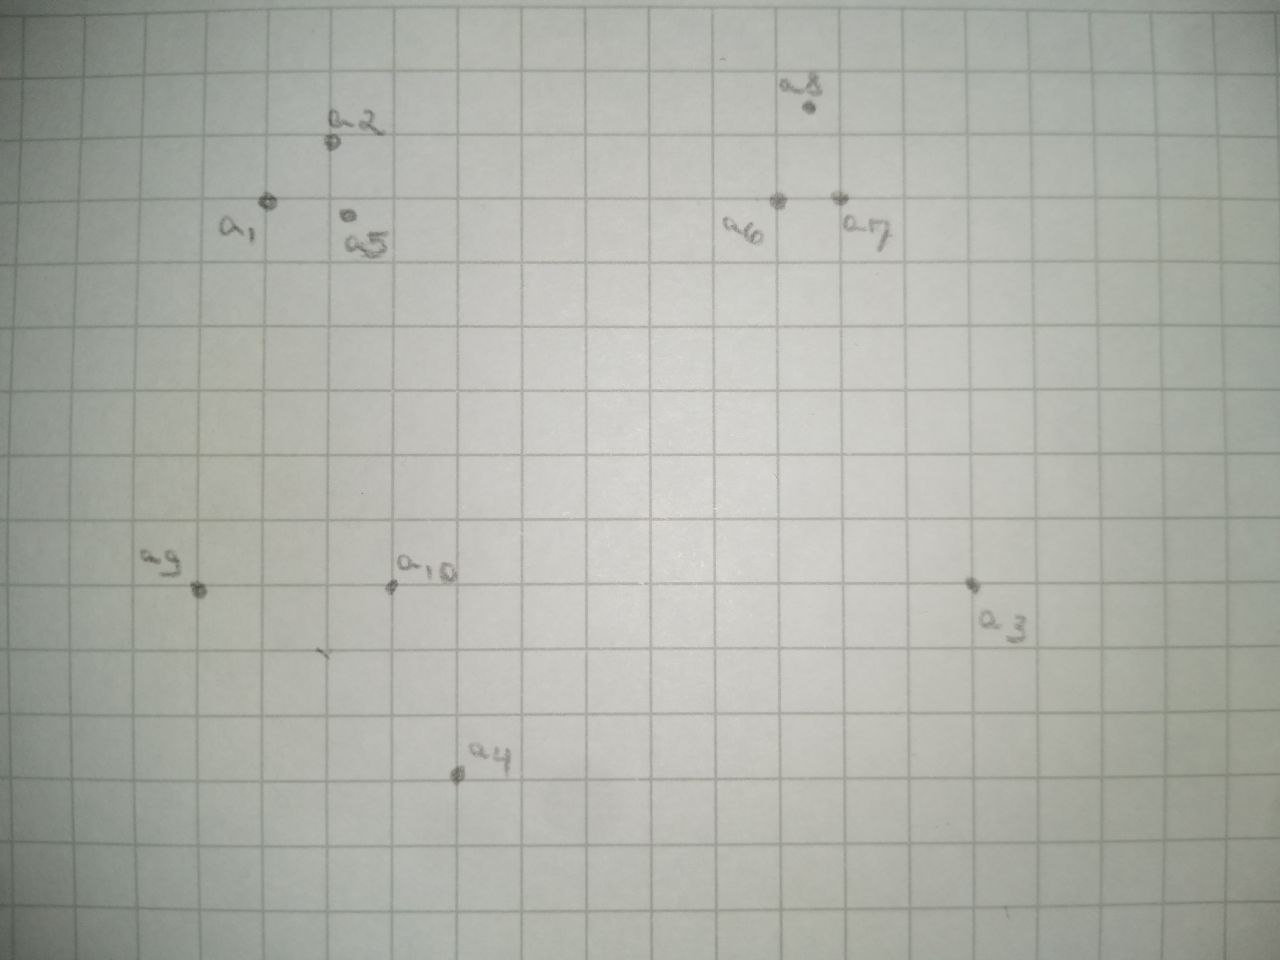
\includegraphics[width=.9\textwidth]{images/q7.jpg}
    \end{center}
\end{exe}

\begin{exe}{8}
    \begin{question}
        (Coeficiente de Rayleign) Calcule:
        \[
            \max_x \frac{ x^T A x }{ x^T x }
        \]
        onde:
        \[
            A \in \R^{n \times n}
            \qquad\text{,}\qquad
            A = A^T
            \qquad\text{e}\qquad
            x \in \R^n
        \]
    \end{question}

    Derivando expressão interna de \(\max\) em relação à \(x\)
    e igualando a \(0\) (para achar pontos críticos):
    \begin{align*}
        &\frac{d}{dx} \frac{ x^T A \; x }{ x^T x } = 0 \\
        &\frac{d}{dx} \left( (x^T A \; x) \; \frac{1}{ x^T x } \right) = 0 \\
        &\left( 2 \; A \; x \; \frac{1}{ x^T x } \right)
            + \left( (x^T A \; x) \; \frac{1}{ (x^T x)^2 } \; (-2 \; x) \right) = 0 \\
        &\frac{
                2 \; (x^T x) \; A \; x
                - 2 \; (x^T A \; x) \; x
            }{ (x^T x)^2 } = 0 \\
        & (x^T x) \; A \; x - (x^T A \; x) \; x = 0 \\
        & ((x^T x) \; A - (x^T A \; x) \; I) \; x = 0
    \end{align*}

    \note{eu fiz mais um pouco mas parece
    que não chegou a lugar algum.}

    Como \(A = A^T\), temos os autovalores e
    seus autovetores associados,
    respectivamente, \(\lambda_1, \dots, \lambda_n\) e
    \(b_1, \dots, b_n\),
    e também que para
    \(0 < i, j \le n\):
    se \(i \ne j\), \(b_i^T b_j = 0\) e
    se \(i = j\), \(b_i^T b_j = 1\).
    Com isso,
    podemos escrever \(x\) como combinação linear deles:
    \[
        x = \sum_{i=0}^n c_i \; b_i
        \qquad,\; c_i \in \R
    \]
    Dessa forma:
    \begin{align*}
        & \left(
                \left(\left(\sum_{i=0}^n c_i \; b_i\right)^T \left(\sum_{i=0}^n c_i \; b_i\right)\right) \; A
                - \left(\left(\sum_{i=0}^n c_i \; b_i\right)^T A \; \left(\sum_{i=0}^n c_i \; b_i\right)\right) \; I
            \right) \; \left(\sum_{i=0}^n c_i \; b_i\right) = 0 \\
        & \left(
                \left(\sum_{i=0}^n \sum_{j=0}^n (c_i \; b_i)^T (c_j \; b_j)\right) \; A
                - \left(\left(\sum_{i=0}^n c_i \; b_i\right)^T \left(\sum_{i=0}^n \lambda_i \; c_i \; b_i\right)\right) \; I
            \right) \; \left(\sum_{i=0}^n c_i \; b_i\right) = 0 \\
        & \left(
                \left(\sum_{i=0}^n \sum_{j=0}^n c_i \; c_j \; {b_i}^T b_j\right) \; A
                - \left(\sum_{i=0}^n \sum_{j=0}^n (c_i \; b_i)^T (\lambda_j \; c_j \; b_j)\right) \; I
            \right) \; \left(\sum_{i=0}^n c_i \; b_i\right) = 0 \\
        & \left(
                \left(\sum_{i=0}^n c_i^2\right) \; A
                - \left(\sum_{i=0}^n \sum_{j=0}^n c_i \; \lambda_j \; c_j \; {b_i}^T b_j\right) \; I
            \right) \; \left(\sum_{i=0}^n c_i \; b_i\right) = 0 \\
        & \left(
                \left(\sum_{i=0}^n c_i^2\right) \; A
                - \left(\sum_{i=0}^n \lambda_i \; c_i^2 \right) \; I
            \right) \; \left(\sum_{i=0}^n c_i \; b_i\right) = 0 \\
        &  \left(\sum_{i=0}^n c_i^2\right) \; A \; \left(\sum_{i=0}^n c_i \; b_i\right)
            - \left(\sum_{i=0}^n \lambda_i \; c_i^2 \right) \; I \; \left(\sum_{i=0}^n c_i \; b_i\right)
            = 0 \\
        &  \left(\sum_{i=0}^n c_i^2\right) \; \left(\sum_{i=0}^n \lambda_i \; c_i \; b_i\right)
            - \left(\sum_{i=0}^n \lambda_i \; c_i^2 \right) \; \left(\sum_{i=0}^n c_i \; b_i\right)
            = 0 \\
        &  \left(\sum_{i=0}^n c_i^2\right) \; \left(\sum_{i=0}^n \lambda_i \; c_i \; b_i\right)
            = \left(\sum_{i=0}^n \lambda_i \; c_i^2 \right) \; \left(\sum_{i=0}^n c_i \; b_i\right)
    \end{align*}
\end{exe}

\begin{exe}[Lista]{1}
    \begin{question}
        Num país politicamente instável,
        \(30\%\) dos defensores da república
        passam a apoiar a monarquia a cada ano e
        \(20\%\) dos defensores da monarquia
        passam a apoiar a república a cada ano.
        Portanto, denotando por \(r_k\) e \(m_k\)
        o número de republicanos e monarquistas,
        respectivamente, no ano k.
        \begin{exe-list}
            \item
                Qual é o código para calcular
                \(r_k\) e \(m_k\)?
            \item
                Sabendo que hoje metade da população
                apoia a república,
                em 10 anos
                qual será o percentual que apoia a república?
            \item
                A longo prazo qual será
                o percentual de republicanos e monarquistas?
        \end{exe-list}
    \end{question}

    \begin{exe-list}
        \item
            Sendo
            \[
                A = \frac{1}{10} \; \begin{bmatrix}
                    7 & 2 \\
                    3 & 8
                \end{bmatrix}
            \]
            temos que
            \[
                \begin{bmatrix}
                    r_k \\ m_k
                \end{bmatrix}
                = A^k \;
                \begin{bmatrix}
                    r_0 \\ m_0
                \end{bmatrix}
            \]
        \item
            \[
                \begin{bmatrix}
                    r_0 \\ m_0
                \end{bmatrix}
                = \begin{bmatrix}
                    0.5 \\ 0.5
                \end{bmatrix}
                \qquad\text{e}\qquad
                k = 10
            \]

            Jogando no J:
            \begin{verbatim}
   (2 2 $ 0.7 0.2 0.3 0.8) (+/ . *)^:10 (2 $ 0.5 0.5)
0.400098 0.599902
            \end{verbatim}

            Então após 10 anos teremos aproximadamente
            \(40\%\) da população apoiando a república.
        \item
            No equilíbrio, teremos que:
            \begin{align*}
                \begin{bmatrix}
                        r \\ m
                    \end{bmatrix} &= A \; \begin{bmatrix}
                        r \\ m
                    \end{bmatrix} \\
                \begin{bmatrix}
                        1 & 0 \\
                        0 & 1
                    \end{bmatrix} \begin{bmatrix}
                        r \\ m
                    \end{bmatrix} &= \frac{1}{10} \; \begin{bmatrix}
                        7 & 2 \\
                        3 & 8
                    \end{bmatrix} \; \begin{bmatrix}
                        r \\ m
                    \end{bmatrix} \\
                0 &= \frac{1}{10} \; \begin{bmatrix}
                        7 & 2 \\
                        3 & 8
                    \end{bmatrix} \; \begin{bmatrix}
                        r \\ m
                    \end{bmatrix} - \begin{bmatrix}
                        1 & 0 \\
                        0 & 1
                    \end{bmatrix} \begin{bmatrix}
                        r \\ m
                    \end{bmatrix} \\
                0 &= \frac{1}{10} \; \begin{bmatrix}
                        7 & 2 \\
                        3 & 8
                    \end{bmatrix} \; \begin{bmatrix}
                        r \\ m
                    \end{bmatrix} - \frac{1}{10} \; \begin{bmatrix}
                        10 & 0 \\
                        0 & 10
                    \end{bmatrix} \begin{bmatrix}
                        r \\ m
                    \end{bmatrix} \\
                0 &= \frac{1}{10} \; \left(
                    \begin{bmatrix}
                        7 & 2 \\
                        3 & 8
                    \end{bmatrix} - \begin{bmatrix}
                        10 & 0 \\
                        0 & 10
                    \end{bmatrix}
                    \right) \; \begin{bmatrix}
                        r \\ m
                    \end{bmatrix} \\
                0 &= \frac{1}{10} \begin{bmatrix}
                        -3 & 2 \\
                        3 & -2
                    \end{bmatrix}
                    \; \begin{bmatrix}
                        r \\ m
                    \end{bmatrix} \\
                0 &= \begin{bmatrix}
                        -3 & 2 \\
                        3 & -2
                    \end{bmatrix}
                    \; \begin{bmatrix}
                        r \\ m
                    \end{bmatrix} \\
                &\begin{cases}
                        -3 r + 2 m &= 0 \\
                        3 r - 2 m &= 0
                    \end{cases} \\
                3 r - 2 m &= 0 \\
                3 r &= 2 m \\
                r &= \frac23 m
            \end{align*}

            Usando que \(r + m = 1\):
            \begin{align*}
                r + m &= 1 \\
                \frac23 m + m &= 1 \\
                2 m + 3 m &= 3 \\
                5 m &= 3 \\
                m &= \frac35 = \frac{6}{10} = 60\% \\
                r &= \frac25 = \frac{4}{10} = 40\%
            \end{align*}

            Jogando no J (\verb._. é infinito):
            \begin{verbatim}
   (2 2 $ 0.7 0.2 0.3 0.8) (+/ . *)^:_ (2 $ 0.5 0.5)
0.4 0.6
            \end{verbatim}
    \end{exe-list}
\end{exe}

\begin{exe}[Lista]{2}
    \begin{question}
        Sequência de Fibonacci. \medskip\noindent\par
        A sequência de Fibonacci
        é definida pelas fórmulas:
        \begin{align*}
            F_0 &= 0 \\
            F_1 &= 1 \\
            F_{t+1} &= F_t + F_{t-1}
        \end{align*}
        Os \(13\) primeiros números da sequência são
        \(0, 1, 1, 2, 3, 5, 6, 13, 21, 34, 55, 89, 144\).

        Esta famosa sequência tem uma profunda conexão
        com o número irracional \(\phi\),
        conhecido como Proporção Áurea.
        Esta proporção possui a seguinte propriedade geométrica:

        \todo{incluir desenho}
        \[
            \frac{a}{b} = \phi = \frac{a+b}{a}
        \]
        \begin{exe-list}
            \item
                Seja
                \[
                    v = \begin{bmatrix}
                        F_t \\ F_{t+1}
                    \end{bmatrix}
                \]
                um vetor cuja primeira coordenada é
                um elemento da sequência e
                a segunda coordenada é o elemento seguinte.
                Determine qual é a matriz \(A\) que
                avança o vetor \(v\) ao longo da sequência,
                ou seja,
                \[
                    A \; v
                    = A \; \begin{bmatrix}
                        F_t \\ F_{t+1}
                    \end{bmatrix}
                    = \begin{bmatrix}
                        F_{t+1} \\ F_{t+2}
                    \end{bmatrix}
                \]
            \item
                Determine os autovetores e autovalores
                da matriz \(A\).
                Sabendo que o resultado da aplicação repetida
                de uma transformação linear
                tende ao autovetor de maior autovalor associado
                daquela transformação
                (\emph{Método da Potência}),
                escreva em Português o que
                os autovetores e autovalores nos dizem
                sobre a Sequência de Fibonacci e
                sua relação com a Proporção Áurea.
            \item
                Dada a lista de números
                da Sequência de Fibonacci acima,
                confira se as conclusões às quais você chegou
                no item anterior se verificam.
        \end{exe-list}
    \end{question}

    \begin{exe-list}
        \item
            \[
                A = \begin{bmatrix}
                    0 & 1 \\
                    1 & 1
                \end{bmatrix}
            \]
        \item
            Seja \(p\) um autovetor de \(A\):
            \begin{align*}
                \lambda \; p &= A \; p \\
                0 &= A \; p - \lambda \; p \\
                0 &= (A - \lambda \; I) \; p \\
                0 &= \left(\begin{bmatrix}
                    0 & 1 \\
                    1 & 1
                \end{bmatrix} - \lambda \; \begin{bmatrix}
                    1 & 0 \\
                    0 & 1
                \end{bmatrix}\right) \; p \\
                0 &= \begin{bmatrix}
                    - \lambda & 1 \\
                    1 & 1 - \lambda
                \end{bmatrix} \; p \\
                &\begin{cases}
                    - \lambda \; a + b &= 0 \\
                    a + (1 - \lambda) \; b &= 0
                \end{cases} \\
                0 &= b + \lambda \; (1 - \lambda) \; b \\
                0 &= (1 + \lambda \; (1 - \lambda)) \; b \\
                0 &= (1 + \lambda \; - \lambda^2) \; b \\
                0 &= 1 + \lambda \; - \lambda^2 \\
                \lambda &= \frac{-1 \pm \sqrt{1 - 4 \; (-1) \; 1}}{-2} \\
                \lambda &= \frac{1 \mp \sqrt{5}}{2}
            \end{align*}

            Os autovetores são:
            \[
                p_+ = x \; \begin{bmatrix}
                    1 \\ \frac{1 + \sqrt{5}}{2}
                \end{bmatrix}
                \qquad\text{e}\qquad
                p_- = x \; \begin{bmatrix}
                    1 \\ \frac{1 - \sqrt{5}}{2}
                \end{bmatrix}
            \]
            onde \(x \in \R\).

            Quanto mais se aplica \(A\)
            a um \(v\) arbitrário,
            mais próximo se chega ao \(p_+\)
            (\emph{Método da Potência}).
            Pela construção de \(A\),
            temos que:
            \[
                \begin{bmatrix}
                    F_{t+1} \\ F_t + F_{t+1}
                \end{bmatrix} = A \;
                \begin{bmatrix}
                    F_t \\ F_{t+1}
                \end{bmatrix}
            \]
            e eventualmente (após aplicar várias vezes)
            vamos chegar à:
            \begin{align*}
                &\begin{bmatrix}
                        F_{t+1} \\ F_t + F_{t+1}
                    \end{bmatrix} = \lambda_+ \; \begin{bmatrix}
                        F_t \\ F_{t+1}
                    \end{bmatrix} \\
                &\begin{cases}
                        \lambda \; F_t &= F_{t+1} \\
                        \lambda \; F_{t+1} &= F_t + F_{t+1}
                    \end{cases} \\
                &\begin{cases}
                        \lambda &= \frac{F_{t+1}}{F_t} \\
                        \lambda &= \frac{F_t + F_{t+1}}{F_{t+1}}
                    \end{cases} \\
                \lambda &= \frac{F_{t+1}}{F_t} = \frac{F_t + F_{t+1}}{F_{t+1}} \\
                \lambda &= \frac{a}{b} = \frac{b + a}{a}
            \end{align*}
            Em outras palavras,
            a Sequência de Fibonacci calcula valores
            que aproximam a Proporção Áurea;
            \(\lambda_+\) é a própria Proporção.

        \item
            Usando J:
            \begin{verbatim}
   ((}. (% ,. [ % +) }:)) 0 1 1 2 3 5 8 13 21 34 55 89 144
      _        1
      1      0.5
      2 0.666667
    1.5      0.6
1.66667    0.625
    1.6 0.615385
  1.625 0.619048
1.61538 0.617647
1.61905 0.618182
1.61765 0.617978
1.61818 0.618056
1.61798 0.618026
   (1 + %: 5) % 2
1.61803
            \end{verbatim}
            A primeira coluna representa \(\frac{a}{b}\) e
            a segunda coluna representa \(\frac{a+b}{a}\).
            Eles vão convergindo para o mesmo valor
            (\(\lambda_+ = \frac{1 + \sqrt{5}}{2} \approx 1.61803\)).
    \end{exe-list}
\end{exe}

\begin{exe}[Lista]{3}
    \begin{question}
        População de bactérias. \medskip\noindent\par
        A população de uma certa espécie de bactéria
        pode ser compreendida da seguinte maneira.
        Existem bactérias novas, maduras e velhas.
        A cada mês:
        \begin{list}{\(\bullet\) (\arabic{exe-list})}{\usecounter{exe-list}}
            \addtocounter{exe-list}{-1}
            \item
                \(80\%\) das bactérias novas
                chegam à maturidade, e
                \(20\%\) morrem;
            \item
                \(50\%\) das bactérias maduras
                tornam-se velhas, e
                \(50\%\) morrem;
            \item
                \(100\%\) das bactérias velhas morrem;
            \item
                Uma a cada duas bactérias maduras
                geram uma nova bactéria;
            \item
                Uma a cada cinco bactérias velhas
                geram uma nova bactéria.
        \end{list}

        \begin{exe-list}
            \item
                Modele o sistema populacional descrito acima --
                ou seja, determine o significado de
                cada coordenada do vetor que representa a população
                em um dado mês,
                e a matriz que representa
                a transição de um mês para o seguinte.
        \end{exe-list}
    \end{question}

    As coordenadas do vetor \(v\) representam,
    as bactérias novas \(v_n\),
    as bactérias maduras \(v_m\),
    as bactérias velhas \(v_v\):
    \[
        v = \begin{bmatrix}
            v_n \\ v_m \\ v_v
        \end{bmatrix}
    \]

    A matrix de transição \(A\) é dada por
    \[
        A = \frac{1}{100} \; \begin{bmatrix}
            0 & 50 & 20 \\
            80 & 0 & 0 \\
            0 & 50 & 0
        \end{bmatrix}
    \]
\end{exe}

\begin{exe}[Lista]{8}
    \begin{question}
        Sejam
        \[
            x = \begin{bmatrix}
                0 \\ 1
            \end{bmatrix}
            \qquad\text{e}\qquad
            A = \begin{bmatrix}
                2 & 1 \\ 1 & 2
            \end{bmatrix}
        \]
        Determine uma aproximação para \(\frac{z_1}{z_2}\),
        tal que \(z = A^{1 \, 000 \, 000} \; x\).
    \end{question}

    A razão \(\frac{z_1}{z_2}\) pode ser aproximada
    pelo maior \(\lambda\) (\emph{Método da Potência}).
    Seja \(p\) um autovetor de \(A\):
    \begin{align*}
        \lambda \; p &= A \; p \\
        0 &= (A - \lambda \; I) \; p \\
        0 &= A \; p - \lambda \; p \\
        0 &= \left(\begin{bmatrix}
            2 & 1 \\
            1 & 2
        \end{bmatrix} - \lambda \; \begin{bmatrix}
            1 & 0 \\
            0 & 1
        \end{bmatrix}\right) \; p \\
        0 &= \begin{bmatrix}
            2 - \lambda & 1 \\
            1 & 2 - \lambda
        \end{bmatrix} \; p \\
        &\begin{cases}
            (2 - \lambda) \; p_1 + p_2 &= 0 \\
            p_1 + (2 - \lambda) \; p_2 &= 0
        \end{cases} \\
        0 &= p_1 - (2 - \lambda)^2 \; p_1 \\
        0 &= (1 - (2 - \lambda)^2) \; p_1 \\
        0 &= (1 - 4 + 4 \; \lambda - \lambda^2) \; p_1 \\
        0 &= (- 3 + 4 \; \lambda - \lambda^2) \; p_1 \\
        0 &= - 3 + 4 \; \lambda - \lambda^2 \\
        \lambda &= \frac{-4 \pm \sqrt{16 - 4 \; (-1) \; (-3)}}{-2} \\
        \lambda &= \frac{4 \mp \sqrt{4}}{2} \\
        \lambda &= \frac{4 \mp 2}{2} \\
        \lambda &= 2 \mp 1 \\
        \lambda &\in \{ 1, 3 \}
    \end{align*}

    Dessa forma:
    \[
        p_+ = x \; \begin{bmatrix}
            1 \\ 1
        \end{bmatrix}
        \qquad\text{e}\qquad
        p_- = x \; \begin{bmatrix}
            1 \\ - 1
        \end{bmatrix}
    \]
    onde \(x \in \R\).

    E a aproximação para \(\frac{z_1}{z_2}\) é \(1\).
\end{exe}

\end{document}
